%% ===============================================================================================
%% @author Leonardo Florez-Valencia (florez-l@javeriana.edu.co)
%% @author David Enrique Palacios García (david_palacios@javeriana.edu.co)
%% @author Karen Sofía Coral Godoy (corallg_ksofia@javeriana.edu.co)
%% ===============================================================================================

\documentclass[letter]{article}

\usepackage[spanish]{babel}
\usepackage[margin=1in]{geometry}
\usepackage{amsmath}
\usepackage{amsthm}
\usepackage{amssymb}
\usepackage[utf8]{inputenc}
\usepackage{graphicx, color}
\usepackage{algorithm}
\usepackage{algpseudocode}
\usepackage{mathrsfs}
\graphicspath{ {graphics/} }
% Some definitions
\floatname{algorithm}{Algoritmo}

% Author info
\title{Escritura del problema del ordenamiento de datos}
\author{David Enrique Palacios García$^1$ \and Karen Sofia Coral Godoy$^1$}
\date{
	$^1$Departamento de Ingeniería de Sistemas, Pontificia Universidad Javeriana\\Bogotá,  Colombia \\
	\texttt{\{david\_palacios, corallg\_ksofia\}@javeriana.edu.co}\\~\\
	\today
}

\begin{document}
\maketitle
	
\begin{abstract}
En este documento se presenta la formalización del problema de ordenamiento de datos, junto con la descripción de tres algoritmos que lo solucionan. Además, se presenta un análisis experimental de la complejidad de esos tres algoritmos.
\textbf{Palabras clave:} ordenamiento, algoritmo, formalización, experimentación, complejidad.
\end{abstract}

\tableofcontents
	
\section{Introducción} \label{intro}
Los algoritmos de ordenamiento de datos son muy útiles en una cantidad considerable de algoritmos que requieren orden en los datos que serán procesados. En este documento se presentan tres de ellos, con el objetivo de mostrar: la formalización del problema (sección \ref{formalizacion}), la escritura formal de tres algoritmos (sección \ref{algoritmos}) y un análisis experimental de la complejidad de cada uno de ellos (sección \ref{experimentos}).

\section{Formalización del problema} \label{formalizacion}
Cuando se piensa en el {\it ordenamiento de números} la solución inmediata puede ser muy simplista: inocentemente, se piensa en ordenar números. Sin embargo, con un poco más de reflexión, hay tres preguntas que pueden surgir:
\begin{enumerate}
  \item ¿Cuáles números?
  \item ¿Cómo se guardan esos números en memoria?
  \item ¿Solo se pueden ordenar números?
\end{enumerate}

Recordemos que los números pueden ser naturales ($\mathbb{N}$), enteros ($\mathbb{Z}$), racionales o quebrados ($\mathbb{Q}$), irracionales ($\mathbb{I}$) y complejos ($\mathbb{C}$). En todos esos conjuntos, se puede definir la relación de {\it orden parcial} $a<b$.

Esto lleva a pensar: si se puede definir la relación de orden parcial $a<b$ en cualquier conjunto $\mathbb{T}$, entonces se puede resolver el problema del ordenamiento con elementos de dicho conjunto.

\subsection{Definición del problema del ``ordenamiento de datos''} \label{problema}
Así, el problema del ordenamiento se define a partir de:
  \begin{enumerate}
    \item una secuencia $S$ de elementos $a\in \mathbb{T}$ y
    \item una relación de orden parcial $a<b~\forall a,b\in \mathbb{T}$
  \end{enumerate}
producir una nueva secuencia $S'$ cuyos elementos contiguos cumplan con la relación $a<b$.
\begin{itemize}
    \item Entradas:
    \begin{itemize}
        \item $S = \left< a_i \in \mathbb{T} \right> ~ | ~ 1\le i \le n$.
        \item $a<b \in \mathbb{T} \times \mathbb{T}$, una relación de orden parcial.
    \end{itemize}
    \item Salidas:
    \begin{itemize}
        \item $S' = \left< e_i \in S m\right> ~ | ~ e_i < e_{i+1} \forall i \in \left[1,n\right)$.
    \end{itemize}
\end{itemize}

\section{Algoritmos de solución} \label{algoritmos}
\subsection{Burbuja ``inocente''} \label{algoritmos:inocente}
La idea de este algoritmo es: comparar todos las parejas de elementos adyacentes e intercambiarlos si no cumplen con la relación de orden parcial $<$.

\begin{algorithm}[!htb]
\caption{Ordenamiento por burbuja ``inocente''.}
\begin{algorithmic}[1]
\Require $S=\left< s_i \in \mathbb{T} \right> \land a<b \in \mathbb{T} \times \mathbb{T}$
\Ensure $S$ será cambiado por $S' = \left< e_i \in S  ~ | ~ e_i < e_{i+1} \forall i \in \left[1,n\right)\right>$
\Procedure{NaiveBubbleSort}{$S$}
  \For{$i \leftarrow 1~\mathbf{to}~|S|$}
    \For{$j \leftarrow 1~\mathbf{to}~|S|-1$}
      \If{$s_{j+1}<s_j$}
        \State \Call{Swap}{$s_j,s_{j+1}$}
      \EndIf
    \EndFor
  \EndFor
\EndProcedure
\end{algorithmic}
\end{algorithm}

\subsubsection{Análisis de complejidad} \label{algoritmos:inocente:complejidad}

Por inspección de código: hay dos ciclos {\it para-todo} anidados que, en el peor de los casos, recorren todo la secuencia de datos; entonces, este algoritmo es $O(|S|^2)$.

\subsubsection{Invariante} \label{algoritmos:inocente:invariante}

Después de cada iteración controlada por el contador $i$, los $i$ elementos más grandes quedan al final de la secuencia.

\begin{enumerate}
    \item Inicio: $i=0$, la secuencia vacía está ordenada.
    \item Iteración: $1 \le i<|S|$, si se supone que los $i-1$ elementos más grandes ya están en su posición, entonces la nueva iteración llevará los $i$-ésimo elemento a su posición adecuada.
    \item Terminación: $i=|S|$, los $|S|$ elementos más grandes están en su posición, entonces la secuencia está ordenada.
\end{enumerate}

\subsection{Burbuja ``mejorado''} \label{algoritmos:mejorado}

La idea de este algoritmo es: comparar todos las parejas de elementos adyacentes e intercambiarlos si no cumplen con la relación de orden parcial $<$, con la diferencia que las comparaciones se detienen en el momento que se alcanzan los elementos más grandes que ya están en su posición final.

\begin{algorithm}[!htb]
\caption{Ordenamiento por burbuja ``mejorado''.}
\begin{algorithmic}[1]
\Require $S=\left< S_i \in \mathbb{T} \right> \land a<b \in \mathbb{T} \times \mathbb{T}$
\Ensure $S$ será cambiado por $S' = \left< e_i \in S  ~ | ~ e_i < e_{i+1} \forall i \in \left[1,n\right)\right>$
\Procedure{ImprovedBubbleSort}{$S$}
  \For{$i \leftarrow 1~\mathbf{to}~|S|$}
    \For{$j \leftarrow 1~\mathbf{to}~|S|-i$} \Comment{Mejora: parar cuando se encuentren los elementos más grandes.}
      \If{$s_{j+1}<s_j$}
        \State \Call{Swap}{$s_j,s_{j+1}$}
      \EndIf
    \EndFor
  \EndFor
\EndProcedure
\end{algorithmic}
\end{algorithm}

\subsubsection{Análisis de complejidad} \label{algoritmos:mejorado:complejidad}

Por inspección de código: hay dos ciclos {\it para-todo} anidados que, en el peor de los casos, recorren todo la secuencia de datos; entonces, este algoritmo es $O(|S|^2)$.

\subsubsection{Invariante} \label{algoritmos:mejorado:invariante}

Después de cada iteración controlada por el contador $i$, los $i$ elementos más grandes quedan al final de la secuencia.

\begin{enumerate}
    \item Inicio: $i=0$, la secuencia vacía está ordenada.
    \item Iteración: $1 \le i<|S|$, si se supone que los $i-1$ elementos más grandes ya están en su posición, entonces la nueva iteración llevará los $i$-ésimo elemento a su posición adecuada.
    \item Terminación: $i=|S|$, los $|S|$ elementos más grandes están en su posición, entonces la secuencia está ordenada.
\end{enumerate}

\subsection{Inserción} \label{algoritmos:insercion}

La idea de este algoritmo es: en cada iteración, buscar la posición donde el elemento que se está iterando quede en el orden de secuencia adecuado.

\begin{algorithm}[!htb]
\caption{Ordenamiento por inserción.}
\begin{algorithmic}[1]
\Require $S=\left< S_i \in \mathbb{T} \right> \land a<b \in \mathbb{T} \times \mathbb{T}$
\Ensure $S$ será cambiado por $S' = \left< e_i \in S m\right> ~ | ~ e_i < e_{i+1} \forall i \in \left[1,n\right)$
\Procedure{InsertionSort}{$S$}
  \For{$j \leftarrow 2~\mathbf{to}~|S|$}
    \State $k \leftarrow s_j$
    \State $i \leftarrow j - 1$
    \While{$0<i \land k < s_i$}
      \State $s_{i+1} \leftarrow s_i$
      \State $i \leftarrow i - 1$
    \EndWhile
    \State $s_{i+1} \leftarrow k$
  \EndFor
\EndProcedure
\end{algorithmic}
\end{algorithm}

\subsubsection{Análisis de complejidad} \label{algoritmos:insercion:complejidad}

Por inspección de código: hay dos ciclos (un {\it mientras-que} anidado dentro de un ciclo {\it para-todo}) anidados que, en el peor de los casos, recorren todo la secuencia de datos; entonces, este algoritmo es $O(|S|^2)$.

El ciclo interior, por el hecho de ser {\it mientras-que}, puede que en algunas configuraciones no se ejecute (i.e. cuando la secuencia ya esté ordenada); entonces, este algoritmo tiene una cota inferior $\Omega(|S|)$, dónde solo el {\it para-todo} recorre la secuencia.

\subsubsection{Invariante} \label{algoritmos:insercion:invariante}

Después de cada iteración $j$, los primeros $j$ siguen la relación de orden parcial $a<b$.

\begin{enumerate}
    \item Inicio: $j \le 1$, la secuencia vacía o unitaria está ordenada.
    \item Iteración: $2 \le j < |S|$, si se supone que los $j-1$ elementos ya están ordenados, entonces la nueva iteración llevará un nuevo elemento y los $j$ primeros elementos estarán ordenados.
    \item Terminación: $j=|S|$, los $|S|$ primeros elementos están ordenados, entonces la secuencia está ordenada.
\end{enumerate}

\section{Análisis experimental} \label{experimentos}

En esta sección se presentarán algunos los experimentos para confirmar los órdenes de complejidad de los tres algoritmos presentados en la sección \ref{algoritmos}.

\subsection{Secuencias aleatorias} \label{experimentos:aleatorias}

Acá se presentan los experimentos cuando los algoritmos se ejecutan con secuencias de entrada de orden aleatorio.

\subsubsection{Protocolo}
\begin{enumerate}
    \item Cargar en memoria un archivo de, al menos, 200Kb.
    \item Definir un rango $(b,e,s)\in\mathbb{N}^3$, donde: $b$ es un tamaño inicial, $e$ es un tamaño final y $s$ es un salto. Se generarán secuencias, a partir del archivo de entrada, de diferentes tamaños desde $b$ hasta $e$, adicionando cada vez $s$ elementos.
    \item Cada algoritmo se ejecutará 5 veces con cada secuencia y se guardará el tiempo promedio de ejecución.
    \item Se generan los gráficos necesarios para comparar los algoritmos.
\end{enumerate}

\subsubsection{Experimentación}
\begin{enumerate}
    \item Se utilizó el programa \texttt{$run\_random\_experiment.py$} con los parámetros de entrada:
    \begin{itemize}
        \item \texttt{paisajeMedio.webp} con un peso de \texttt{345KB} como archivo de entrada
        \item \texttt{b=0} como tamaño inicial del arreglo
        \item \texttt{e=10000} como tamaño final del arreglo
        \item \texttt{s=100} como saltos entre iteraciones del algoritmo
    \end{itemize}
    \item El programa logró finalizar sin complicaciones, con un tiempo estimado de 2 horas.
    \item Se obtuvieron 100 datos con el tiempo promedio de cada uno de los algoritmos, logrando así crear la siguiente gráfica: (ver Figura 1)
\end{enumerate}

\begin{figure}[h]
    \centering
    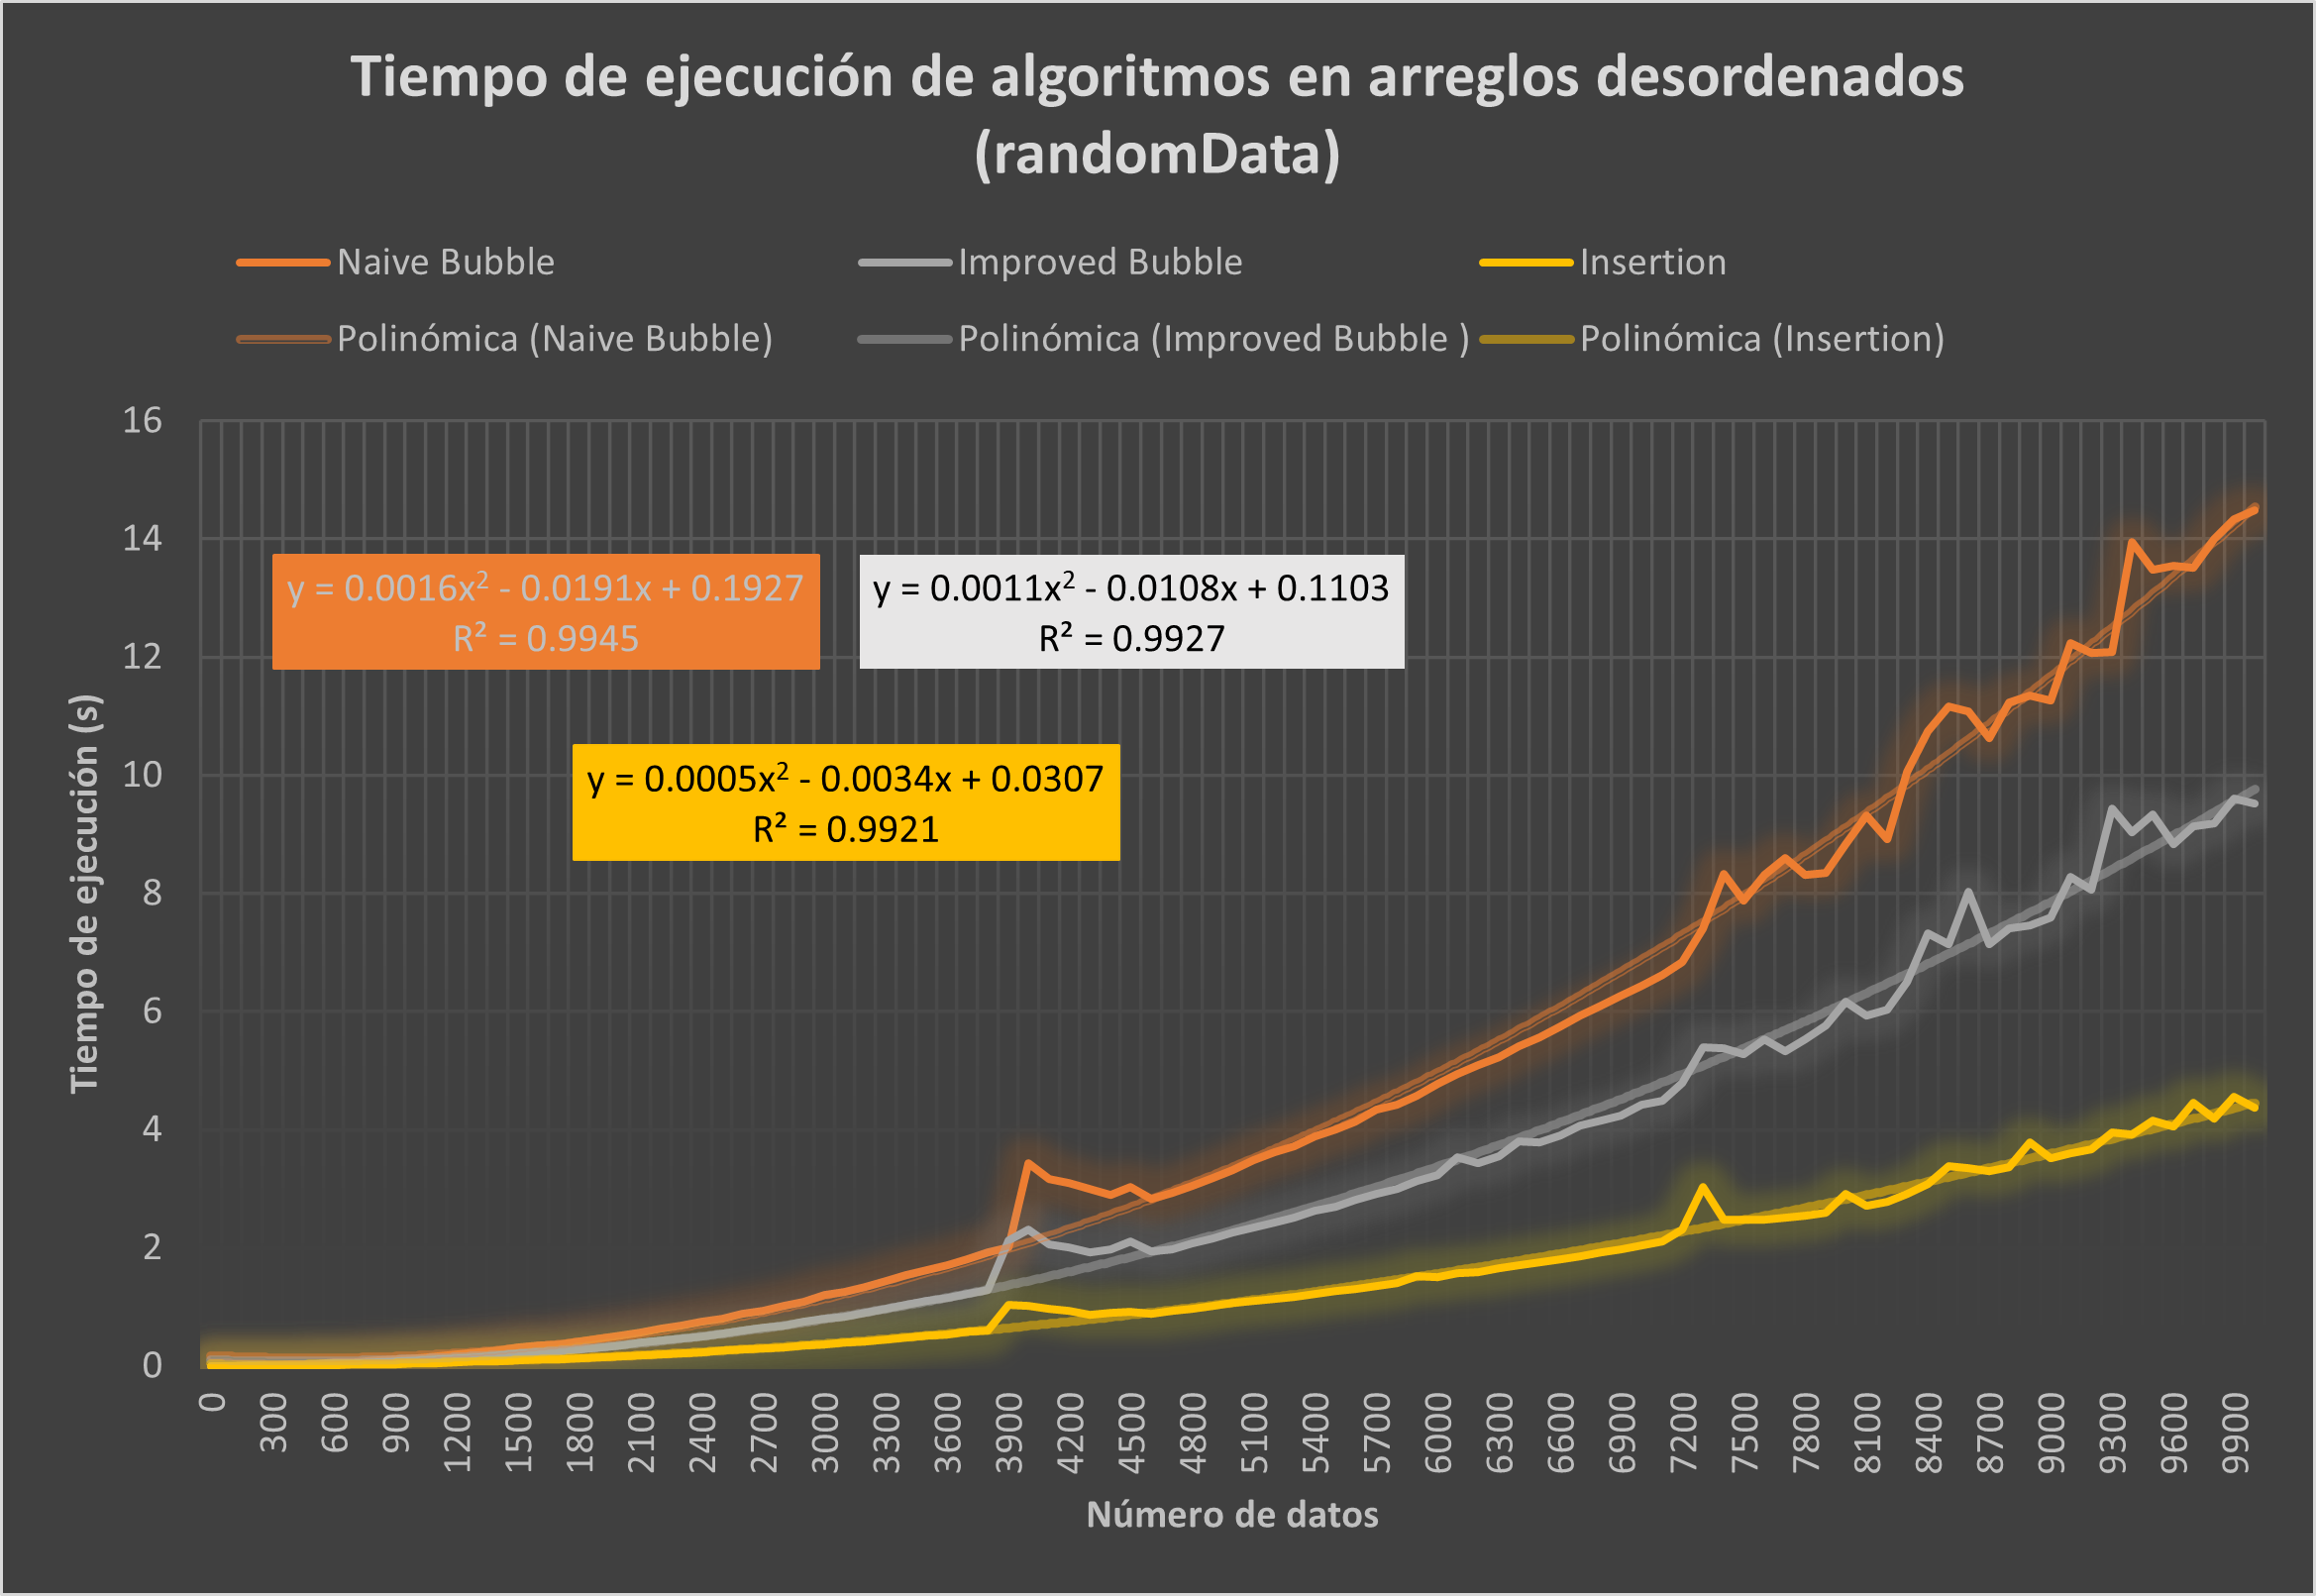
\includegraphics[scale=0.90]{randomDataGraphic.png}
    \label{experimentos:aleatorias:grafica}
    \caption{Tiempo de ejecución de los algoritmos con datos desordenados}
\end{figure}

\subsubsection{Análisis del experimento}
\label{experimentos:aleatorias:analisis}
Como se puede notar, en este caso los 3 algoritmos tienen una complejidad $\Theta(n^{2})$, sin embargo, a partir de arreglos de 1500 datos, se empiezan a notar diferencias entre ellos. La principal es que es evidente que, aunque no deja de ser cuadrática, el Insertion Sort es mucho más rápido que el Bubble Sort Inocente y su contraparte mejorada. Eso sí, también se nota la mejoría del Bubble Sort aplicando la correción estudiada anteriormente.

Así mismo, aplicando herramientas de Microsoft Excel, se pudo obtener las fórmulas de las regresiones cuadráticas de estos algoritmos, confirmando así su tendencia hacia $n^2$.

\subsection{Secuencias ordenadas} \label{experimentos:ordenadas}

Acá se presentan los experimentos cuando los algoritmos se ejecutan con secuencias de entrada ordenadas de acuerdo al orden parcial $a<b$.

\subsubsection{Protocolo}
\begin{enumerate}
    \item Definir un rango $(b,e,s)\in\mathbb{N}^3$, donde: $b$ es un tamaño inicial, $e$ es un tamaño final y $s$ es un salto. Se generarán secuencias aleatorias de diferentes tamaños desde $b$ hasta $e$, adicionando cada vez $s$ elementos.
    \item Se usará el algoritmo \texttt{sort(S)}, disponible en la librería básica de python, para ordenar dicha secuencia.
    \item Cada algoritmo se ejecutará 5 veces con cada secuencia ordenada y se guardará el tiempo promedio de ejecución.
    \item Se generan los gráficos necesarios para comparar los algoritmos.
\end{enumerate}

\subsubsection{Experimentación}
\begin{enumerate}
    \item Se utilizó el programa \texttt{$run\_sorted\_experiment.py$} con los parámetros de entrada:
    \begin{itemize}
        \item \texttt{b=0} como tamaño inicial del arreglo
        \item \texttt{e=10000} como tamaño final del arreglo
        \item \texttt{s=100} como saltos entre iteraciones del algoritmo
    \end{itemize}
    \item Se creó un arreglo de tamaño \texttt{e} con números aleatorios entre -1000000 y 1000000.
    \item Utilizando la función \texttt{sort(S)} de la librería básica de Pyhton, se ordena ascendentemente el arreglo y se empiezan a ejecutar los algoritmos. 
    \item El programa logró finalizar sin complicaciones, con un tiempo estimado de hora y media.
    \item Se obtuvieron 100 datos con el tiempo promedio de cada uno de los algoritmos, logrando así crear la siguiente gráfica: (ver Figura 2)
\end{enumerate}

\begin{figure}[h]
    \centering
    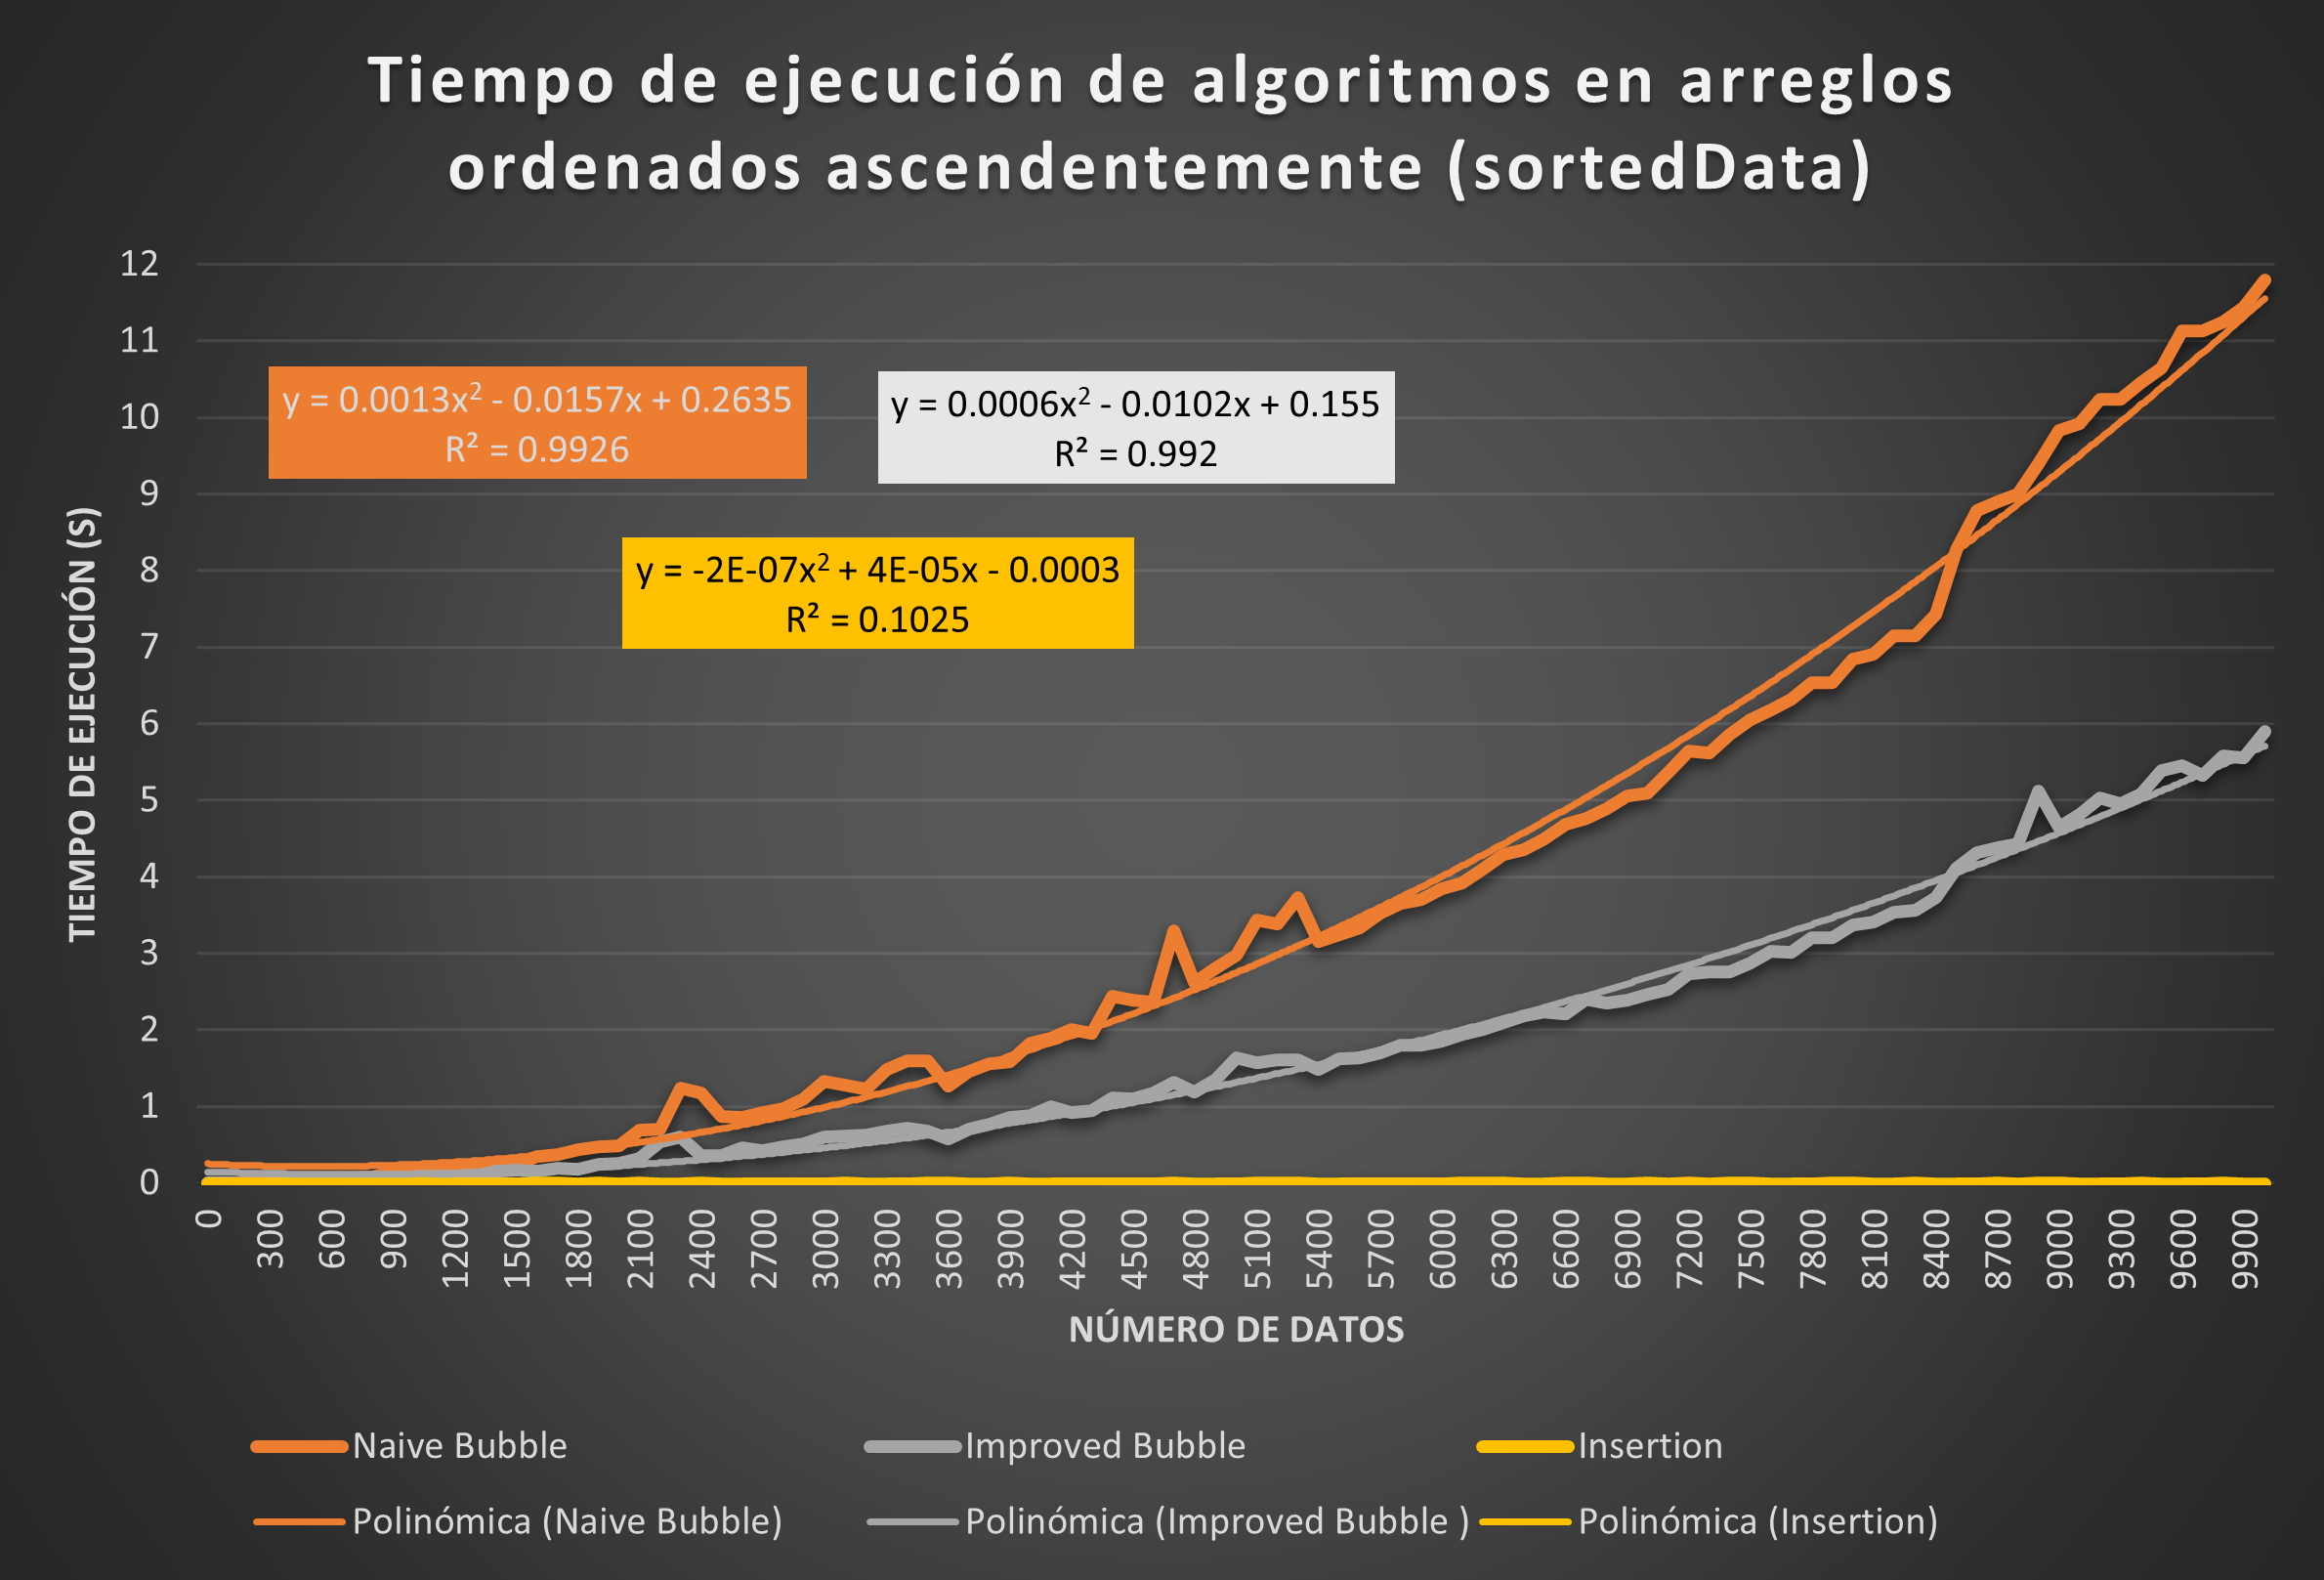
\includegraphics[scale=0.9]{sortedDataGraphic.png}
    \caption{Tiempo de ejecución de los algoritmos con datos ordenados ascendentemente}
   \label{experimentos:ordenadas:grafica}
\end{figure}


\subsubsection{Análisis del experimento}
\label{experimentos:ordenadas:analisis}
Una vez más, podemos notar la complejidad $\Theta(n^2)$ para Bubble Sort en sus dos variantes; no obstante, se mejora bastante el tiempo de ejecucicón, pues pasa de un máximo de 14 segundos a uno de aproximádamente 12 segundos.

Por otra parte, es clave notar el mejor caso posible para Insertion Sort.El hecho de que sea casi tangente al eje x nos demuestra que su cota de complejidad inferior se cumple, siendo $\Omega(n)$.

Además, haciendo el análisis de regresión de las curvas, notamos que el Insertion Sort no deja de ser cuadrática, sin embargo, la constante que acompaña al $x^2$ es $-2^{-7}$, lo que lo hace tender a 0. Esto ocasiona que se convierta en una función lineal, muy cercana al eje horizontal de la gráfica.


\subsection{Secuencias ordenadas invertidas} \label{experimentos:invertidas}

Acá se presentan los experimentos cuando los algoritmos se ejecutan con secuencias de entrada ordenadas de forma invertida de acuerdo al orden parcial $a<b$.

\subsubsection{Protocolo}
\begin{enumerate}
    \item Definir un rango $(b,e,s)\in\mathbb{N}^3$, donde: $b$ es un tamaño inicial, $e$ es un tamaño final y $s$ es un salto. Se generarán secuencias aleatorias de diferentes tamaños desde $b$ hasta $e$, adicionando cada vez $s$ elementos.
    \item Se usará el algoritmo \texttt{sort(S)} con el parámetro \texttt{reverse=True}, disponible en la librería básica de python, para ordenar dicha secuencia de manera descendente.
    \item Cada algoritmo se ejecutará 5 veces con cada secuencia ordenada y se guardará el tiempo promedio de ejecución.
    \item Se generan los gráficos necesarios para comparar los algoritmos.
\end{enumerate}

\subsubsection{Experimentación}
\begin{enumerate}
    \item Se utilizó el programa \texttt{$run\_reverse\_sorted\_experiment.py$} con los parámetros de entrada:
    \begin{itemize}
        \item \texttt{b=0} como tamaño inicial del arreglo
        \item \texttt{e=10000} como tamaño final del arreglo
        \item \texttt{s=100} como saltos entre iteraciones del algoritmo
    \end{itemize}
    \item Se creó un arreglo de tamaño \texttt{e} con números aleatorios entre -1000000 y 1000000.
    \item Utilizando la función \texttt{sort(S)} de la librería básica de Pyhton, junto con el parámetro \texttt{reverse=True}, se ordena descendentemente el arreglo y se empiezan a ejecutar los algoritmos. 
    \item El programa logró finalizar sin complicaciones, con un tiempo estimado de 2 horas y media.
    \item Se obtuvieron 100 datos con el tiempo promedio de cada uno de los algoritmos, logrando así crear la siguiente gráfica: (ver Figura 3)
\end{enumerate}

\begin{figure}[h]
    \centering
    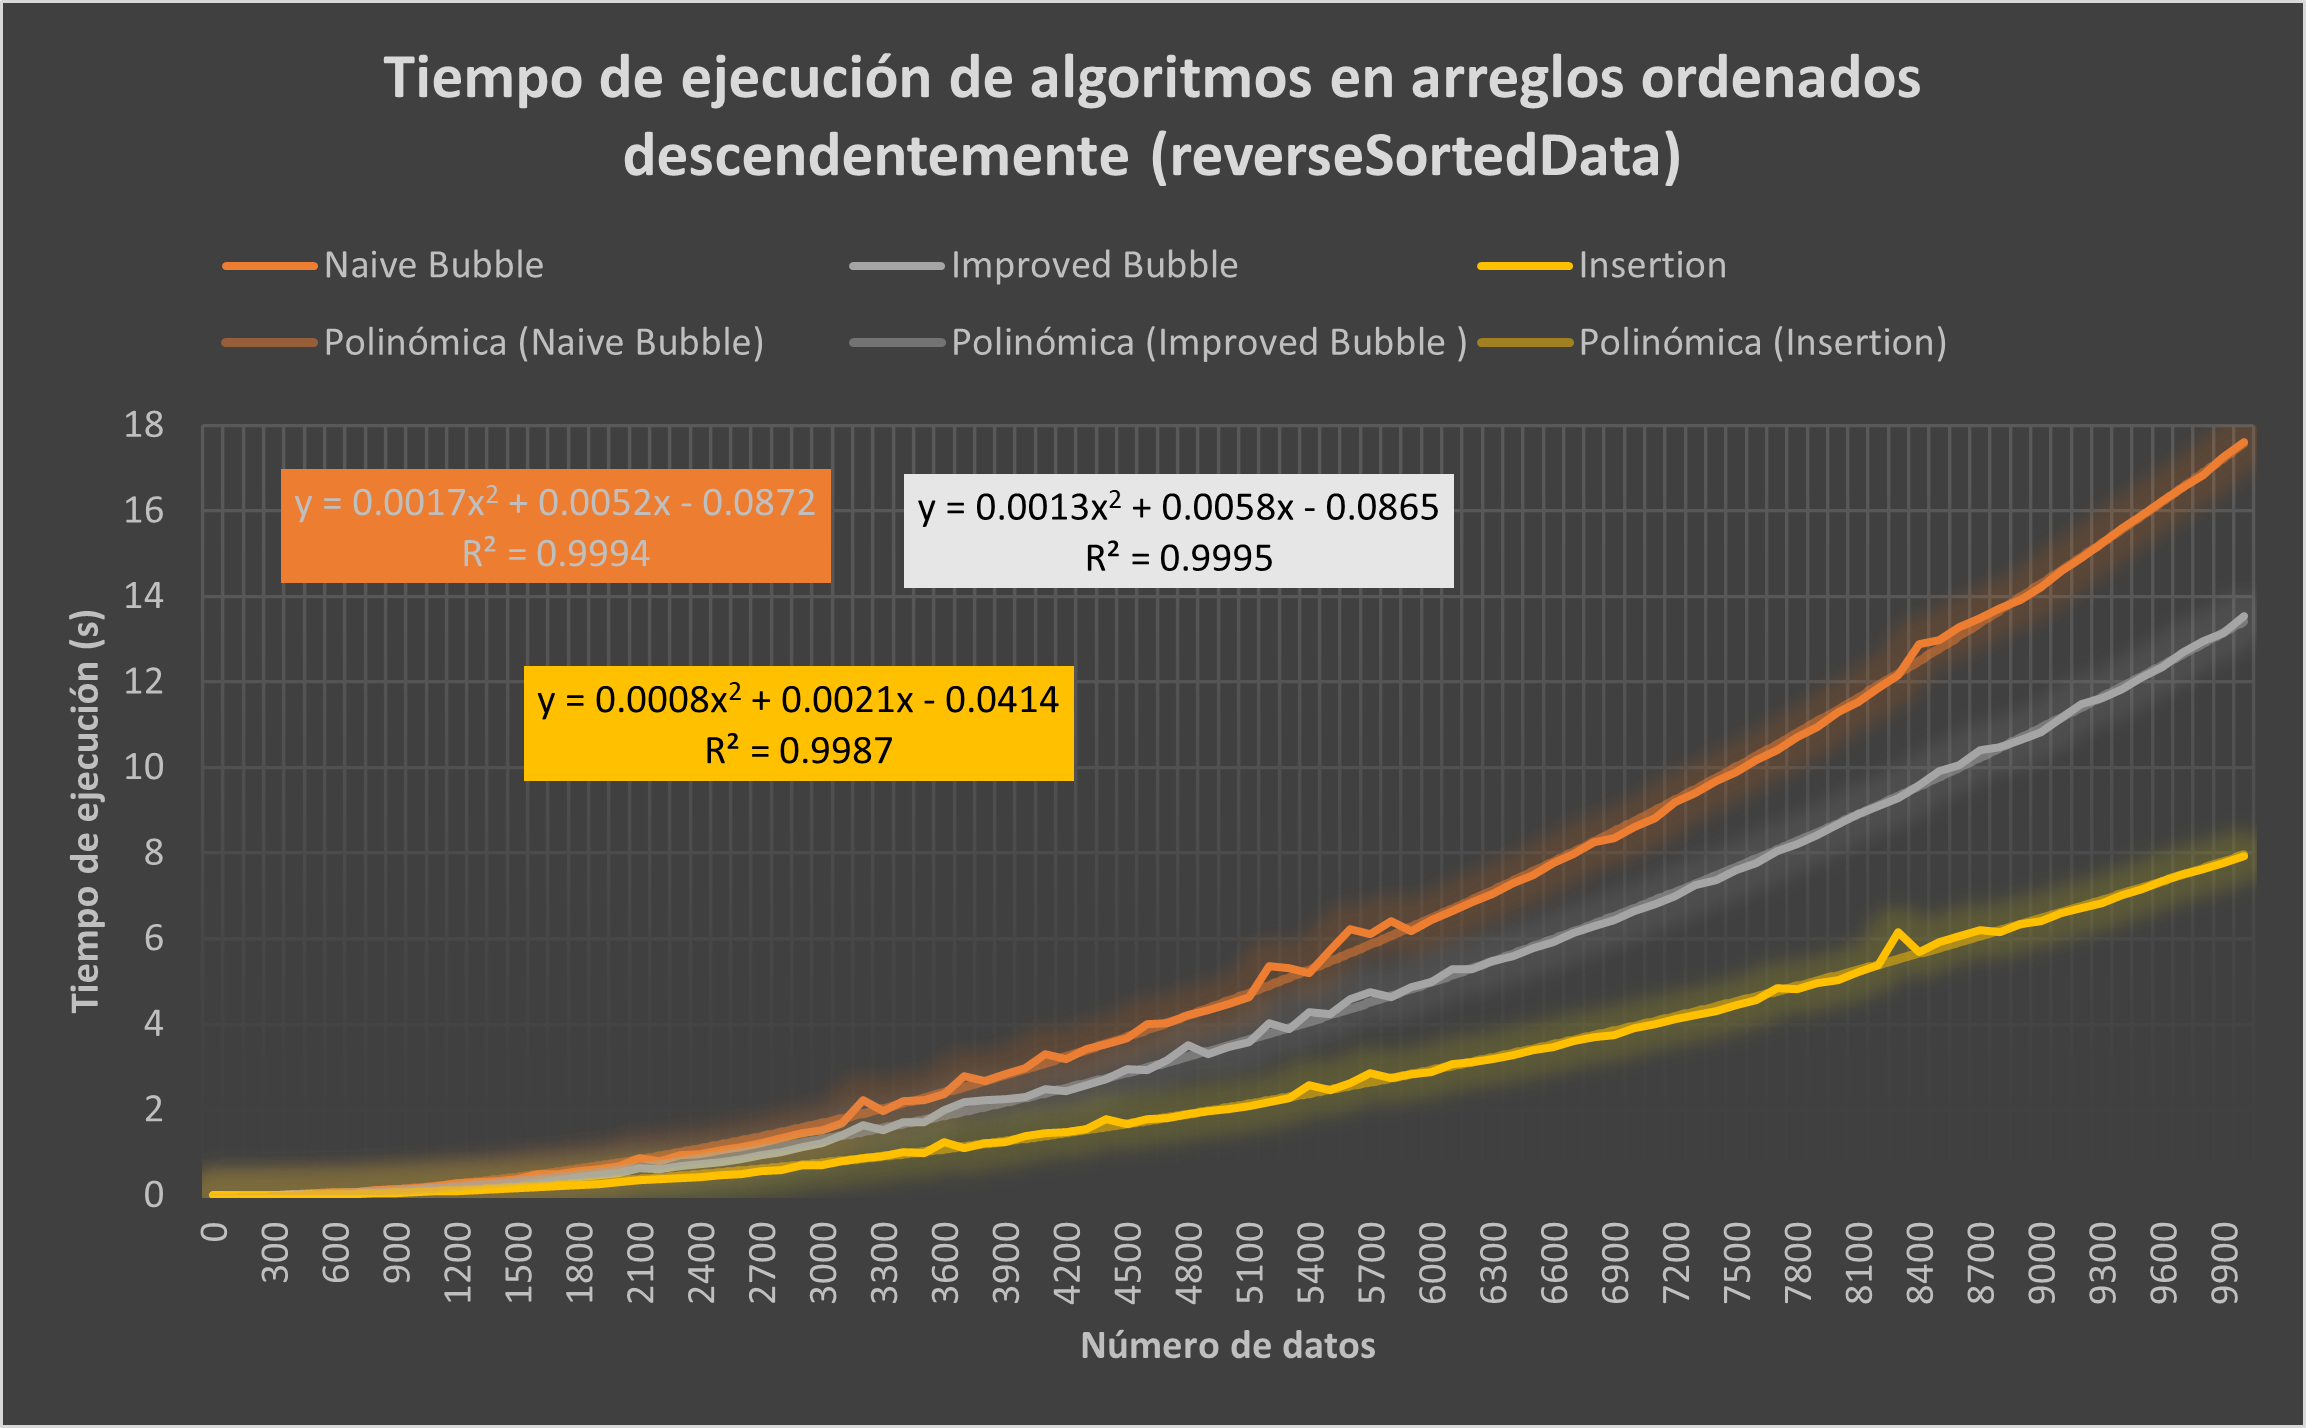
\includegraphics[scale=1]{reverseSortedDataGraphic.png}
    \caption{Tiempo de ejecución de los algoritmos con datos ordenados descendentemente}
   \label{experimentos:invertidas:grafica}
\end{figure}


\subsubsection{Análisis del experimento}
\label{experimentos:invertidas:analisis}
Para los 3 algoritmos, este fue el peor escenario posible. Es aquí donde las iteraciones tomaron más tiempo para lograr ordenar los arreglos. Esto ocurre por la invariante de los algoritmos, donde, en el caso de Bubble Sort se busca ubicar los valores más grandes hacia el final del arreglo, y en Insertion Sort, en el que se ajustan primero los menores valores.

Es interesante cuestionarse qué tipo de algoritmo implementa \texttt{sort(S)} de Python, pues únicamente añadiendo el parámetro \texttt{reverse=True}, efectúa el ordenamiento descendente de manera casi instantánea.

Investigando un poco en internet, se encontró que, \cite{Ed} desde la versión 2.3 de Python, éste usa el TimSort para ordenar los datos. Este algoritmo tiene una complejidad de $O(nlogn)$ siendo así uno basado en la estrategia de divide y vencerás, logrando su objetivo a velocidades prácticamente imperceptibles.

\section{Conclusiones}
Los experimentos fueron útiles para concluir:
\begin{enumerate}
    \item El tiempo de ejecución para el caso promedio (datos aleatorios) de estos algoritmos tiene una complejidad de $\Theta(n^2)$
    \item Insertion Sort tiene una cota de complejidad de $\Omega(n)$ si el arreglo está previamente ordenado de manera ascendente.
    \item Para todos los algoritmos, el peor caso es cuando el arreglo está previamente ordenado de manera descendente. Aquí, la cota de complejidad es $O(n^2)$.
    \item Los algoritmos estudiados en este taller funcionan de manera educativa para aprender sobre complejidad algorítmica, pero no deberían ser usados en un proyecto real. En ese caso, se podría optar por otros como el TimSort o el HeapSort.
\end{enumerate}

\begin{thebibliography}{X}
\bibitem{Ed} \textsc{Educative IO},
\textit{What is the Python list sort()?}, https://www.educative.io/answers/what-is-the-python-list-sort

\end{thebibliography}



\end{document}

%% eof - sorting.tex
